\documentclass[11pt,a4paper]{article}

% === Packages ===
\usepackage[utf8]{inputenc}
\usepackage[T1]{fontenc}
\usepackage{amsmath,amssymb,amsfonts}
\usepackage{graphicx}
\usepackage{booktabs}
\usepackage{hyperref}
\usepackage{listings}
\usepackage{xcolor}
\usepackage{algorithm}
\usepackage{algpseudocode}
\usepackage{multirow}
\usepackage{enumitem}
\usepackage{url}
\usepackage{natbib}
\usepackage{geometry}
\geometry{margin=1in}

% === Code Listing Styles ===
\definecolor{splkeyword}{RGB}{0,0,180}
\definecolor{splstring}{RGB}{163,21,21}
\definecolor{splcomment}{RGB}{0,128,0}
\definecolor{splbuiltin}{RGB}{128,0,128}
\definecolor{codebg}{RGB}{248,248,248}

\lstdefinelanguage{SPL}{
  keywords={PROMPT, WITH, BUDGET, TOKENS, USING, MODEL, SELECT, AS, LIMIT,
            WHERE, AND, OR, NOT, IN, ORDER, BY, ASC, DESC, GENERATE, OUTPUT,
            CREATE, FUNCTION, RETURNS, EXPLAIN, EXECUTE, PARAMS, STORE, RESULT,
            CACHE, FOR, FROM, TEMPERATURE, FORMAT},
  keywordstyle=\color{splkeyword}\bfseries,
  morekeywords=[2]{system_role, context, rag, memory},
  keywordstyle=[2]{\color{splbuiltin}\bfseries},
  sensitive=false,
  morecomment=[l]{--},
  commentstyle=\color{splcomment}\itshape,
  morestring=[b]",
  morestring=[b]',
  stringstyle=\color{splstring},
  basicstyle=\ttfamily\small,
  breaklines=true,
  showstringspaces=false,
  tabsize=4,
  frame=single,
  backgroundcolor=\color{codebg},
  captionpos=b,
}

\lstdefinestyle{python}{
  language=Python,
  basicstyle=\ttfamily\small,
  keywordstyle=\color{splkeyword}\bfseries,
  stringstyle=\color{splstring},
  commentstyle=\color{splcomment}\itshape,
  breaklines=true,
  showstringspaces=false,
  frame=single,
  backgroundcolor=\color{codebg},
}

\lstdefinestyle{ebnf}{
  basicstyle=\ttfamily\small,
  breaklines=true,
  frame=single,
  backgroundcolor=\color{codebg},
}

% === Title ===
\title{%
  \textbf{Structured Prompt Language:\\
  Declarative Context Management for LLMs}
}

\author{
  Wen Gong\\
  \small \texttt{wen.gong.research@gmail.com}
}

\date{February 2026}

\begin{document}

\maketitle

% ============================================================
\begin{abstract}
% ============================================================

We present \textbf{SPL} (Structured Prompt Language), a declarative, SQL-inspired query language for managing LLM context as a constrained resource. Just as SQL (1970) standardized access to relational databases, SPL standardizes interactions with large language models by treating them as \emph{generative knowledge bases}---systems that not only store but actively synthesize knowledge. SPL introduces explicit \emph{token budget management} through declarative \texttt{WITH BUDGET} and \texttt{LIMIT} clauses, \emph{automatic context optimization} via a query optimizer that allocates tokens across heterogeneous sources, and \emph{execution plan transparency} through an \texttt{EXPLAIN} mechanism analogous to SQL's query plan. The language natively integrates retrieval-augmented generation (RAG) via FAISS vector stores and persistent memory via SQLite, unifying context retrieval, generation, and storage in a single declarative framework. We provide a formal EBNF grammar, a complete reference implementation as a pip-installable Python package, and a comparative analysis against existing approaches including Microsoft's Prompty, Stanford's DSPy, and LMQL. Our evaluation demonstrates that SPL reduces prompt engineering complexity while providing fine-grained control over the token budget---the fundamental constrained resource in LLM applications.

\end{abstract}

\textbf{Keywords:} large language models, prompt engineering, declarative languages, context management, token optimization, retrieval-augmented generation

% ============================================================
\section{Introduction}
\label{sec:intro}
% ============================================================

The emergence of large language models (LLMs) as general-purpose reasoning engines has created an unprecedented challenge in software engineering: \emph{how to systematically manage the context window}---the fixed-size input buffer that determines what information an LLM can consider when generating responses. Context window sizes range from 4K tokens in early models to over 1M tokens in recent architectures, yet the challenge remains fundamentally the same: context is a \emph{constrained resource} that must be allocated efficiently across competing demands.

The current state of LLM prompt engineering bears a striking resemblance to database programming before SQL. In the pre-SQL era (1960s), programmers wrote imperative, procedural code to navigate data structures---each database vendor had its own access methods, and there was no standard way to express \emph{what} data was needed versus \emph{how} to retrieve it. Codd's relational model~\citep{codd1970relational} and the subsequent development of SQL~\citep{chamberlin1974sequel} resolved this chaos by introducing a declarative language that separated logical queries from physical execution.

Today's prompt engineers face an analogous problem:

\begin{itemize}[nosep]
  \item \textbf{Manual token counting}: Developers hand-calculate whether their prompts fit within context windows, often through trial and error.
  \item \textbf{Ad hoc truncation}: When context exceeds limits, engineers apply crude truncation strategies with no systematic optimization.
  \item \textbf{No visibility}: There is no standard way to inspect how tokens are allocated across different parts of a prompt.
  \item \textbf{Provider lock-in}: Prompt code is typically tied to specific LLM APIs, making migration costly.
  \item \textbf{No composability}: Unlike SQL's Common Table Expressions (CTEs) and views, prompts are monolithic and resist modular reuse.
\end{itemize}

We propose \textbf{SPL (Structured Prompt Language)}, a declarative query language that applies the principles that made SQL successful---declarative specification, automatic optimization, composability, portability, and transparency---to the domain of LLM context management.

\subsection{The Core Insight: LLM as Generative Knowledge Base}

The key conceptual innovation of SPL is treating an LLM not merely as a function that maps text to text, but as a \emph{generative knowledge base}. Traditional databases are \emph{static} knowledge bases: they store and retrieve data that was explicitly inserted. LLMs, by contrast, encode knowledge implicitly in their trained parameters and can \emph{synthesize} novel content---answers, analyses, code, creative works---that never existed in their training data.

This distinction motivates SPL's dual-clause architecture:
\begin{itemize}[nosep]
  \item \texttt{SELECT} gathers context (analogous to SQL \texttt{SELECT} retrieving data)
  \item \texttt{GENERATE} synthesizes new content (unique to generative knowledge bases)
\end{itemize}

Table~\ref{tab:sql-spl-parallel} formalizes the parallel between SQL and SPL.

\begin{table}[h]
\centering
\caption{The SQL--SPL parallel: from static to generative knowledge bases.}
\label{tab:sql-spl-parallel}
\begin{tabular}{@{}lll@{}}
\toprule
\textbf{Dimension} & \textbf{SQL (1970)} & \textbf{SPL (2026)} \\
\midrule
Knowledge base & Static (rows/tables) & Generative (trained weights) \\
Query result & Retrieved data & Synthesized content \\
Constrained resource & Disk I/O, RAM & Token budget (context window) \\
Optimization goal & Minimize I/O & Minimize tokens, maximize relevance \\
\texttt{SELECT} & Retrieves existing data & Gathers context from sources \\
\texttt{GENERATE} & N/A & Creates new content from context \\
\texttt{EXPLAIN} & Shows query execution plan & Shows token allocation plan \\
CTEs / Views & Compose complex queries & Compose complex prompts \\
Transactions & ACID guarantees & Memory persistence + caching \\
Provider portability & Oracle, Postgres, MySQL & OpenRouter, Claude, GPT, Llama \\
\bottomrule
\end{tabular}
\end{table}

\subsection{Contributions}

This paper makes the following contributions:

\begin{enumerate}[nosep]
  \item \textbf{Language design}: We present the complete syntax and formal grammar (EBNF) of SPL, a declarative language for LLM context management with explicit token budgeting, composable CTEs, user-defined functions, and integrated RAG/memory.
  \item \textbf{Context-as-resource model}: We formalize the LLM context window as a constrained resource and present a token budget allocation algorithm analogous to query optimization in relational databases.
  \item \textbf{EXPLAIN mechanism}: We introduce transparent execution plans for LLM queries, enabling developers to inspect and reason about token allocation before execution.
  \item \textbf{Reference implementation}: We provide a complete, pip-installable Python package (\texttt{spl-llm}) with a hand-written recursive descent parser, optimizer, and provider-agnostic execution engine.
  \item \textbf{Comparative analysis}: We systematically compare SPL against existing prompt management approaches (Prompty, DSPy, LMQL) across key dimensions.
\end{enumerate}

% ============================================================
\section{Background and Motivation}
\label{sec:background}
% ============================================================

\subsection{The Prompt Engineering Problem}

As LLMs have become central to software systems, prompt engineering has emerged as a critical discipline. Developers must construct input sequences that effectively utilize the model's capabilities while respecting hard constraints on context window size and soft constraints on cost and latency.

Current prompt engineering practices are overwhelmingly \emph{imperative}: developers write Python (or JavaScript, etc.) code that concatenates strings, counts tokens, applies heuristic truncation, and makes API calls. This imperative approach has several well-documented problems:

\begin{enumerate}[nosep]
  \item \textbf{Tight coupling}: Prompt construction logic is interleaved with application logic, making prompts difficult to test, version, and share.
  \item \textbf{No budget discipline}: Without explicit budget allocation, developers discover token overflows only at runtime (often in production).
  \item \textbf{Optimization blind spots}: Imperative code obscures the structure of token allocation, making it impossible to reason about whether the budget is spent optimally.
  \item \textbf{Reinvention}: Common patterns (RAG context injection, conversation history management, response caching) are reimplemented from scratch in every project.
\end{enumerate}

These patterns were directly encountered during the development of
Data-Copilot~\citep{gong2024datacopilot}, a RAG-powered conversational analytics
application, and motivated the design of SPL.

\subsection{Lessons from SQL's Success}

SQL has dominated database interaction for over five decades because it embodies a set of principles that proved universally valuable:

\begin{description}[nosep]
  \item[Declarative] Specify \emph{what} you want, not \emph{how} to get it. The optimizer handles execution strategy.
  \item[Optimizable] A query planner can reorder joins, choose indexes, and parallelize---impossible with imperative navigation.
  \item[Composable] CTEs, views, subqueries, and functions enable modular construction of complex queries.
  \item[Portable] The same SQL runs (with minor dialect differences) on Oracle, PostgreSQL, MySQL, SQLite, and hundreds of other engines.
  \item[Transparent] \texttt{EXPLAIN} reveals the execution plan, enabling informed optimization by the developer.
\end{description}

SPL applies each of these principles to LLM context management, as we detail in the following sections.

\subsection{The Token Budget as Constrained Resource}

We propose a formal model of the LLM context window as a constrained resource allocation problem. Given a context window of $B$ tokens, an SPL query must allocate this budget across $n$ context sources $s_1, \ldots, s_n$, a generation task $g$, and a safety buffer $\beta$:

\begin{equation}
\label{eq:budget}
\sum_{i=1}^{n} \text{tokens}(s_i) + \text{tokens}(g) + \beta \leq B
\end{equation}

Each source $s_i$ has:
\begin{itemize}[nosep]
  \item An \emph{estimated size} $\hat{t}_i$ (tokens before optimization)
  \item An optional \emph{limit} $L_i$ (the \texttt{LIMIT} clause)
  \item A \emph{priority} $p_i$ (derived from source type: memory $>$ cache $>$ RAG $>$ context)
  \item A \emph{compression ratio} $c_i \in (0, 1]$ (applied when over budget)
\end{itemize}

The optimizer's task is to find allocations $a_i \leq \min(\hat{t}_i, L_i)$ that satisfy Equation~\ref{eq:budget} while maximizing information utility. This is analogous to the query optimizer in relational databases, which minimizes I/O cost subject to producing correct results.

% ============================================================
\section{The SPL Language}
\label{sec:language}
% ============================================================

\subsection{Design Philosophy}

SPL follows three design principles:

\begin{enumerate}[nosep]
  \item \textbf{SQL familiarity}: Leverage the muscle memory of millions of SQL developers. Anyone who can write \texttt{SELECT ... FROM ... WHERE} can learn SPL quickly.
  \item \textbf{Budget-first}: Every SPL query explicitly states its token budget. This forces developers to think about context allocation upfront, preventing runtime surprises.
  \item \textbf{Source-agnostic}: Context sources (user input, RAG results, memory) are accessed through a uniform interface, making queries composable regardless of where data originates.
\end{enumerate}

\subsection{Core Syntax}

The fundamental SPL statement is the \texttt{PROMPT} query, which has the following structure:

\begin{lstlisting}[language=SPL, caption={Basic SPL query structure}]
PROMPT answer_question
WITH BUDGET 8000 tokens
USING MODEL claude-sonnet-4-5

SELECT
    system_role("You are a knowledgeable assistant"),
    context.question AS question LIMIT 200 tokens,
    rag.query("relevant docs", top_k=5) AS docs LIMIT 3000 tokens,
    memory.get("history") AS history LIMIT 500 tokens

WHERE
    docs.relevance > 0.7

ORDER BY
    docs.relevance DESC

GENERATE
    detailed_answer(question, docs, history)
WITH OUTPUT BUDGET 2000 tokens, TEMPERATURE 0.3, FORMAT markdown;
\end{lstlisting}

The key clauses are:

\begin{description}[nosep]
  \item[\texttt{PROMPT <name>}] Names the query for reuse and reference.
  \item[\texttt{WITH BUDGET <n> tokens}] Declares the total token budget for the entire operation (input + output).
  \item[\texttt{USING MODEL <model>}] Specifies the target LLM, enabling model-specific token counting and cost estimation.
  \item[\texttt{SELECT}] Gathers context from heterogeneous sources, each with an optional \texttt{LIMIT} cap.
  \item[\texttt{WHERE}] Filters context items based on conditions (e.g., relevance thresholds for RAG results).
  \item[\texttt{ORDER BY}] Orders context items, controlling which appear first in the assembled prompt.
  \item[\texttt{GENERATE}] Specifies the generation task with output parameters.
  \item[\texttt{STORE RESULT IN memory.<key>}] Persists results to the memory store for future queries.
\end{description}

\subsection{Built-in Context Sources}

SPL provides four built-in context source types:

\begin{table}[h]
\centering
\caption{SPL built-in context sources.}
\label{tab:sources}
\begin{tabular}{@{}llp{6cm}@{}}
\toprule
\textbf{Source} & \textbf{Syntax} & \textbf{Description} \\
\midrule
System role & \texttt{system\_role("...")} & Sets the system/instruction prompt \\
Context & \texttt{context.<field>} & References external input parameters \\
RAG & \texttt{rag.query("...", top\_k=N)} & Semantic retrieval from vector store \\
Memory & \texttt{memory.get("key")} & Key-value retrieval from persistent store \\
\bottomrule
\end{tabular}
\end{table}

\subsection{Common Table Expressions (CTEs)}

Like SQL, SPL supports CTEs via the \texttt{WITH} clause, enabling composition of complex prompts from simpler building blocks:

\begin{lstlisting}[language=SPL, caption={CTEs for composable prompt construction}]
PROMPT analyze_and_recommend
WITH BUDGET 12000 tokens
USING MODEL claude-sonnet-4-5

WITH compressed_profile AS (
    SELECT
        context.user_profile AS profile
    LIMIT 500 tokens
),
relevant_docs AS (
    SELECT
        rag.query("product recommendations", top_k=3) AS docs
    LIMIT 2000 tokens
)

SELECT
    system_role("You are a product recommendation expert"),
    compressed_profile AS profile,
    relevant_docs AS docs,
    memory.get("purchase_history") AS history LIMIT 1000 tokens

GENERATE
    product_recommendations(profile, docs, history)
WITH OUTPUT BUDGET 4000 tokens, TEMPERATURE 0.5

STORE RESULT IN memory.last_recommendations;
\end{lstlisting}

CTEs serve two purposes: (1) they enable token-limited preprocessing of context sources, and (2) they create reusable named components within a query.

\subsection{User-Defined Functions}

SPL supports \texttt{CREATE FUNCTION} for reusable prompt components:

\begin{lstlisting}[language=SPL, caption={User-defined function}]
CREATE FUNCTION compress_bio(bio, max_tokens)
RETURNS text
AS $$
    SELECT bio LIMIT max_tokens tokens
$$;
\end{lstlisting}

Functions encapsulate common context processing patterns (compression, formatting, extraction) and can be invoked from any \texttt{SELECT} or \texttt{GENERATE} clause.

\subsection{EXPLAIN Mechanism}

The \texttt{EXPLAIN} statement produces a detailed token allocation plan without executing the query:

\begin{lstlisting}[language=SPL, caption={EXPLAIN for execution plan transparency}]
EXPLAIN PROMPT answer_question;
\end{lstlisting}

This produces output such as:

\begin{verbatim}
Execution Plan for: answer_question
============================================================
Budget: 8,000 tokens | Model: claude-sonnet-4-5

Token Allocation:
+-- __system_role__               20 tokens  (  0.2%)
+-- history                      500 tokens  (  6.2%)  [from memory]
+-- docs                       3,000 tokens  ( 37.5%)  [cache MISS]
+-- question                     200 tokens  (  2.5%)
+-- Output Budget              2,000 tokens  ( 25.0%)
\-- Buffer                     2,280 tokens  ( 28.5%)
                               ----------
Total                          5,720 / 8,000 tokens (71.5%)

Estimated Cost: $0.0412
\end{verbatim}

The \texttt{EXPLAIN} output provides: (1) a tree view of token allocation across all context sources, (2) the percentage of budget consumed by each source, (3) cache status for each source, (4) compression annotations where applicable, and (5) estimated cost based on the target model's pricing.

This mechanism is directly analogous to SQL's \texttt{EXPLAIN} / \texttt{EXPLAIN ANALYZE}, which shows query execution plans including join strategies, index usage, and estimated row counts. For LLM queries, the ``execution plan'' is the token allocation strategy.

\subsection{Formal Grammar}

We provide a complete EBNF grammar for SPL. The grammar is context-free and LL(1)-parseable by a recursive descent parser. A condensed version of the core productions:

\begin{lstlisting}[style=ebnf, caption={SPL grammar (condensed EBNF)}]
program        = statement (";" statement)* ";"? EOF ;
statement      = prompt_stmt | create_func_stmt
               | explain_stmt | execute_stmt ;

prompt_stmt    = "PROMPT" IDENT header_clauses cte_block?
                 select_clause where_clause? order_clause?
                 generate_clause store_clause? ;

header_clauses = ("WITH" "BUDGET" INTEGER "TOKENS")?
                 ("USING" "MODEL" (IDENT | STRING))?
                 ("CACHE" "FOR" INTEGER IDENT)? ;

cte_block      = "WITH" cte_def ("," cte_def)* ;
cte_def        = IDENT "AS" "(" select_clause from_clause?
                 where_clause? ("LIMIT" INTEGER "TOKENS")? ")" ;

select_clause  = "SELECT" select_item ("," select_item)* ;
select_item    = source_expr ("AS" IDENT)?
                 ("LIMIT" INTEGER "TOKENS")? ;

source_expr    = "system_role" "(" STRING ")"
               | "context" "." IDENT
               | "rag" "." "query" "(" STRING
                 ("," "top_k" "=" INTEGER)? ")"
               | "memory" "." "get" "(" STRING ")"
               | IDENT "(" arg_list? ")" | IDENT ;

generate_clause = "GENERATE" IDENT "(" arg_list? ")"
                  ("WITH" generate_opt ("," generate_opt)*)? ;
generate_opt    = "OUTPUT" "BUDGET" INTEGER "TOKENS"
                | "TEMPERATURE" FLOAT | "FORMAT" IDENT ;
\end{lstlisting}

The full grammar specification containing all productions (including \texttt{WHERE}, \texttt{ORDER BY}, \texttt{CREATE FUNCTION}, \texttt{EXECUTE}, and expression rules) is provided in the supplementary materials.

% ============================================================
\section{Context as a Constrained Resource}
\label{sec:context-resource}
% ============================================================

\subsection{Information-Theoretic Formulation}

We model an SPL query as a resource allocation problem. Let $\mathcal{Q}$ be an SPL query with total budget $B$, output budget $O$, and context sources $S = \{s_1, \ldots, s_n\}$. The \emph{input budget} available for context is:

\begin{equation}
B_{\text{input}} = B - O - \beta
\end{equation}

where $\beta$ is a safety buffer (typically 5--10\% of $B$).

Each context source $s_i$ has:
\begin{itemize}[nosep]
  \item Raw token count: $t_i = \text{tokens}(s_i)$
  \item User-specified limit: $L_i$ (from \texttt{LIMIT} clause, or $\infty$ if unspecified)
  \item Effective allocation: $a_i = \min(t_i, L_i)$
\end{itemize}

The budget constraint is:
\begin{equation}
\sum_{i=1}^{n} a_i \leq B_{\text{input}}
\end{equation}

When $\sum a_i > B_{\text{input}}$ (over-budget), the optimizer applies proportional compression:
\begin{equation}
a'_i = a_i \cdot \frac{B_{\text{input}}}{\sum_{j=1}^{n} a_j} \quad \text{(proportional scaling)}
\end{equation}

with a refinement: items are compressed largest-first, and items with explicit \texttt{LIMIT} clauses are given priority to retain their specified allocation.

\subsection{Cost Model}

SPL's cost model parallels relational algebra's cost model. In SQL, the optimizer estimates I/O cost (disk pages read, index lookups). In SPL, the optimizer estimates:

\begin{equation}
\text{Cost}(\mathcal{Q}) = \text{cost\_per\_input\_token}(m) \cdot \sum a_i + \text{cost\_per\_output\_token}(m) \cdot O
\end{equation}

where $m$ is the target model. This enables \texttt{EXPLAIN} to display estimated dollar cost before execution, allowing developers to make informed decisions about model selection and budget allocation.

\subsection{Execution Order Optimization}

The SPL optimizer also determines the order in which context sources are resolved, following a priority hierarchy:

\begin{enumerate}[nosep]
  \item \textbf{Cache hits}: Previously computed results (zero latency, zero cost)
  \item \textbf{Memory}: SQLite key-value lookups (sub-millisecond, zero cost)
  \item \textbf{RAG}: FAISS vector search (milliseconds, minimal cost)
  \item \textbf{Context}: External input parameters (variable latency)
  \item \textbf{LLM calls}: The generation step (highest latency and cost)
\end{enumerate}

This ordering minimizes latency by executing the cheapest operations first, analogous to how SQL optimizers prefer index scans over full table scans.

% ============================================================
\section{The SPL Engine}
\label{sec:engine}
% ============================================================

\subsection{Architecture}

The SPL engine follows a classic compiler pipeline architecture, mirroring the structure of SQL query engines:

\begin{verbatim}
SPL Source (.spl file)
       |
   [Lexer]            Character stream -> Token stream
       |
   [Parser]           Token stream -> AST
       |
   [Analyzer]         AST -> Validated AST
       |
   [Optimizer]        Validated AST -> Execution Plan
       |
   [Executor]         Execution Plan -> Results
   /    |    \
[LLM] [Memory] [RAG]
  |       |       |
OpenRouter SQLite  FAISS
\end{verbatim}

\subsubsection{Lexer}

The lexer performs character-by-character scanning, producing a stream of typed tokens. It handles: SQL-style keywords (case-insensitive), string literals (single and double quotes), numeric literals (integer and floating-point), dot notation for qualified references (\texttt{context.field}), \texttt{\$\$} delimiters for function bodies, and \texttt{--} single-line comments. The keyword set includes 30+ reserved words (Table~\ref{tab:keywords}).

\begin{table}[h]
\centering
\caption{SPL keyword categories.}
\label{tab:keywords}
\begin{tabular}{@{}lp{10cm}@{}}
\toprule
\textbf{Category} & \textbf{Keywords} \\
\midrule
Structural & \texttt{PROMPT}, \texttt{SELECT}, \texttt{GENERATE}, \texttt{WITH}, \texttt{AS}, \texttt{FROM} \\
Budget & \texttt{BUDGET}, \texttt{TOKENS}, \texttt{LIMIT}, \texttt{OUTPUT} \\
Model & \texttt{USING}, \texttt{MODEL}, \texttt{TEMPERATURE}, \texttt{FORMAT} \\
Filtering & \texttt{WHERE}, \texttt{AND}, \texttt{OR}, \texttt{NOT}, \texttt{IN}, \texttt{ORDER}, \texttt{BY}, \texttt{ASC}, \texttt{DESC} \\
Functions & \texttt{CREATE}, \texttt{FUNCTION}, \texttt{RETURNS} \\
Control & \texttt{EXPLAIN}, \texttt{EXECUTE}, \texttt{PARAMS}, \texttt{STORE}, \texttt{RESULT}, \texttt{CACHE}, \texttt{FOR} \\
Built-ins & \texttt{system\_role}, \texttt{context}, \texttt{rag}, \texttt{memory} \\
\bottomrule
\end{tabular}
\end{table}

\subsubsection{Parser}

The parser is a hand-written recursive descent parser---a deliberate architectural choice over parser generators (ANTLR, Lark) for three reasons:

\begin{enumerate}[nosep]
  \item \textbf{Zero dependencies}: The parser has no external dependencies, reducing the attack surface and installation friction.
  \item \textbf{Full control}: Error messages can reference SPL-specific concepts (``expected GENERATE clause after SELECT'') rather than generic parse errors.
  \item \textbf{Formalizability}: The one-to-one correspondence between grammar productions and parser methods makes the implementation a direct proof of the grammar's LL(1) property, suitable for inclusion in a formal language specification.
\end{enumerate}

The parser produces a typed AST with dataclass nodes for each syntactic construct (Table~\ref{tab:ast-nodes}).

\begin{table}[h]
\centering
\caption{Core AST node types.}
\label{tab:ast-nodes}
\begin{tabular}{@{}lp{9cm}@{}}
\toprule
\textbf{Node Type} & \textbf{Description} \\
\midrule
\texttt{PromptStatement} & Top-level query with budget, model, select, generate clauses \\
\texttt{SelectItem} & Single context source with optional alias and token limit \\
\texttt{CTEClause} & Common table expression (named subquery) \\
\texttt{GenerateClause} & Generation specification with parameters \\
\texttt{CreateFunctionStatement} & User-defined function definition \\
\texttt{ExplainStatement} & EXPLAIN query \\
\texttt{ExecuteStatement} & Parameterized query execution \\
\bottomrule
\end{tabular}
\end{table}

\subsubsection{Semantic Analyzer}

The analyzer performs validation passes on the AST:

\begin{itemize}[nosep]
  \item \textbf{Name resolution}: Verifies that all referenced aliases (in \texttt{GENERATE} arguments, \texttt{WHERE} conditions) correspond to defined \texttt{SELECT} items or CTEs.
  \item \textbf{Budget arithmetic}: Warns when the sum of \texttt{LIMIT} clauses exceeds the total budget.
  \item \textbf{Type checking}: Validates that context sources are used with correct syntax (e.g., \texttt{rag.query} requires a string argument).
  \item \textbf{Duplicate detection}: Reports duplicate prompt names, aliases, or CTE definitions.
\end{itemize}

\subsubsection{Optimizer}

The optimizer transforms a validated AST into an \texttt{ExecutionPlan}---an ordered sequence of steps with token allocations. The optimization algorithm (Algorithm~\ref{alg:optimizer}) proceeds as follows:

\begin{algorithm}[h]
\caption{SPL Token Budget Optimizer}
\label{alg:optimizer}
\begin{algorithmic}[1]
\Require $B$: total budget, $O$: output budget, $S$: set of SELECT items
\Ensure ExecutionPlan with token allocations
\State $B_{\text{input}} \gets B - O - \beta$
\For{each $s_i \in S$}
  \State $\hat{t}_i \gets \text{estimate\_tokens}(s_i)$
  \State $a_i \gets \min(\hat{t}_i, L_i)$ \Comment{Apply LIMIT cap}
\EndFor
\If{$\sum a_i > B_{\text{input}}$}
  \State Sort $S$ by $a_i$ descending \Comment{Compress largest first}
  \State $\text{excess} \gets \sum a_i - B_{\text{input}}$
  \For{each $s_i$ in sorted order}
    \State $\text{reduction} \gets \min(a_i \times 0.5, \text{excess})$
    \State $a_i \gets a_i - \text{reduction}$
    \State $\text{excess} \gets \text{excess} - \text{reduction}$
    \If{$\text{excess} \leq 0$} \textbf{break} \EndIf
  \EndFor
\EndIf
\State Sort $S$ by priority: memory $>$ cache $>$ RAG $>$ context
\State \Return ExecutionPlan($S$, allocations, cost estimate)
\end{algorithmic}
\end{algorithm}

\subsubsection{Executor}

The executor processes the ExecutionPlan step by step:

\begin{enumerate}[nosep]
  \item Resolve each context source (load from memory, execute RAG queries, read parameters)
  \item Apply token limits via truncation
  \item Check prompt cache (hash-based, with TTL)
  \item Assemble the final prompt string with system role, context sections, and generation instruction
  \item Call the LLM adapter
  \item Optionally store results via \texttt{STORE RESULT IN memory.<key>}
  \item Return structured result with content, token usage, timing, and cost
\end{enumerate}

\subsection{LLM Adapter Interface}

SPL achieves provider-agnosticism through an abstract adapter interface:

\begin{lstlisting}[style=python, caption={LLM adapter interface (Python)}]
class LLMAdapter(ABC):
    @abstractmethod
    async def generate(
        self, prompt: str, model: str,
        max_tokens: int = 4096,
        temperature: float = 0.7,
        system: str | None = None,
    ) -> GenerationResult: ...

    @abstractmethod
    def count_tokens(self, text: str, model: str) -> int: ...

    @abstractmethod
    def list_models(self) -> list[str]: ...
\end{lstlisting}

The reference implementation includes two adapters:

\begin{description}[nosep]
  \item[OpenRouter Adapter] (Production): Calls the OpenRouter.ai API, which provides access to 100+ models (Claude, GPT, Llama, Mistral, Gemini, etc.) through a single unified endpoint. This realizes SPL's vision of provider-agnosticism at the infrastructure level.
  \item[Claude CLI Adapter] (Development): Wraps the Claude Code CLI via subprocess, leveraging subscription-based billing for zero-marginal-cost development. This adapter demonstrates that SPL can interface with any LLM access method, not just HTTP APIs.
\end{description}

\subsection{Storage Layer}

SPL integrates two storage systems, both file-based for portability:

\begin{description}[nosep]
  \item[SQLite Memory Store] (\texttt{.spl/memory.db}): Provides persistent key-value storage for \texttt{memory.get()} and \texttt{STORE RESULT IN memory.<key>}. Also stores prompt cache entries with TTL support. SQLite was chosen for its zero-configuration deployment, battle-tested reliability, and inclusion in the Python standard library.
  \item[FAISS Vector Store] (\texttt{.spl/vectors.faiss}): Provides semantic similarity search for \texttt{rag.query()}. Document metadata is stored in a companion SQLite database (\texttt{.spl/vectors\_meta.db}). FAISS was chosen for its speed, wide adoption, and file-based persistence.
\end{description}

Both stores reside in a \texttt{.spl/} directory within the project, analogous to \texttt{.git/} for version control. This directory is gitignore-able and self-contained, enabling reproducible deployments.

% ============================================================
\section{LLM as Generative Knowledge Base}
\label{sec:generative-kb}
% ============================================================

The deepest contribution of SPL is the conceptual framework of treating LLMs as \emph{generative knowledge bases}. This section elaborates on this framework and its implications.

\subsection{From Retrieval to Synthesis}

Traditional information systems follow a retrieve-and-present paradigm: a user poses a query, the system searches its index, and returns matching documents. The user must then synthesize understanding from the retrieved items.

LLMs break this paradigm. When queried, an LLM does not merely retrieve stored information; it \emph{synthesizes} a novel response by combining:

\begin{enumerate}[nosep]
  \item \textbf{Parametric knowledge}: Information encoded in model weights during training
  \item \textbf{Contextual knowledge}: Information provided in the current prompt (the context window)
  \item \textbf{Reasoning}: Emergent multi-step inference capabilities
\end{enumerate}

SPL's dual-clause architecture (\texttt{SELECT} + \texttt{GENERATE}) directly mirrors this distinction:

\begin{itemize}[nosep]
  \item \texttt{SELECT} populates the contextual knowledge (items 2--3 above)
  \item \texttt{GENERATE} triggers the synthesis process, which draws on all three sources
\end{itemize}

This is why SPL is not merely ``a prompt template language''---it is a \emph{query language for a generative knowledge base}, where the ``database'' (LLM weights) can produce outputs that never existed in its ``tables'' (training data).

\subsection{The Duality with SQL}

In SQL, the \texttt{SELECT} statement both specifies what to retrieve \emph{and} produces the result. In SPL, we separate these concerns:

\begin{itemize}[nosep]
  \item \texttt{SELECT} specifies what context to \emph{gather} (retrieval phase)
  \item \texttt{GENERATE} specifies what to \emph{create} from that context (synthesis phase)
\end{itemize}

This separation enables the optimizer to treat context gathering and generation as distinct phases with different resource characteristics, leading to better budget allocation.

\subsection{Implications for Software Engineering}

Treating LLMs as generative knowledge bases has several implications for software engineering practice:

\begin{enumerate}[nosep]
  \item \textbf{Prompt engineering becomes query engineering}: The skill set shifts from ``crafting text that tricks the model'' to ``declaring what context and what output are needed.''
  \item \textbf{Observability becomes possible}: Just as SQL \texttt{EXPLAIN} enables database performance tuning, SPL \texttt{EXPLAIN} enables prompt performance tuning.
  \item \textbf{Testing becomes structured}: SPL queries can be validated statically (parse, analyze) and their resource usage estimated before any LLM call.
  \item \textbf{Version control becomes meaningful}: \texttt{.spl} files are human-readable, diffable, and reviewable---unlike embedded prompt strings in application code.
\end{enumerate}

% ============================================================
\section{Related Work}
\label{sec:related}
% ============================================================

We compare SPL against existing approaches for managing LLM interactions. Table~\ref{tab:comparison} provides a feature-level comparison; we discuss each approach below.

\begin{table}[h]
\centering
\caption{Feature comparison of LLM prompt management approaches.}
\label{tab:comparison}
\resizebox{\textwidth}{!}{%
\begin{tabular}{@{}lccccc@{}}
\toprule
\textbf{Feature} & \textbf{SPL} & \textbf{LMQL} & \textbf{Prompty} & \textbf{DSPy} & \textbf{LangChain} \\
\midrule
Declarative query language & \checkmark & \checkmark & -- & -- & -- \\
Explicit token budgeting & \checkmark & Partial\textsuperscript{a} & -- & -- & -- \\
EXPLAIN execution plan & \checkmark & -- & -- & -- & -- \\
Built-in RAG & \checkmark & -- & -- & -- & Via plugins \\
Persistent memory & \checkmark & -- & -- & -- & Via plugins \\
SQL-like CTEs \& functions & \checkmark & -- & -- & -- & -- \\
Provider-agnostic & \checkmark & \checkmark & Partial\textsuperscript{b} & \checkmark & \checkmark \\
Automatic compression & \checkmark & -- & -- & -- & -- \\
Formal grammar (EBNF) & \checkmark & \checkmark & -- & -- & -- \\
Zero-dependency parser & \checkmark & -- & N/A & N/A & N/A \\
Prompt optimization & --\textsuperscript{c} & -- & -- & \checkmark & -- \\
SQL knowledge reusable & \checkmark & Partial\textsuperscript{d} & -- & -- & -- \\
\bottomrule
\end{tabular}%
}

\smallskip
\textsuperscript{a} LMQL supports per-variable length constraints but not global budget allocation. \\
\textsuperscript{b} Prompty primarily targets Azure/OpenAI; community adapters exist for others. \\
\textsuperscript{c} SPL optimizes \emph{token allocation} (resource management); DSPy optimizes \emph{prompt content} (few-shot examples). These are complementary, not competing, concerns. \\
\textsuperscript{d} LMQL borrows SQL keywords (\texttt{FROM}, \texttt{WHERE}) for token-level generation constraints, but its mental model differs substantially from relational query thinking. SPL is intentionally modeled on SQL end-to-end, enabling practitioners with SQL experience to adopt GenAI workflows without learning a new programming paradigm.
\end{table}

\subsection{Prompty (Microsoft)}

Prompty~\citep{prompty2024} is Microsoft's approach to standardizing prompt engineering through a YAML-based file format (\texttt{.prompty}). Prompty files declare model parameters, input/output schemas, and template text with variable interpolation. It integrates with Microsoft's Semantic Kernel and Azure AI Foundry ecosystem.

\textbf{Key differences from SPL:}
\begin{itemize}[nosep]
  \item \emph{Template vs.\ query}: Prompty is a \emph{template format}---it defines static prompt structures with variable slots. SPL is a \emph{query language}---it expresses dynamic context gathering, optimization, and generation as a single declarative query.
  \item \emph{No token budgeting}: Prompty relies on the underlying model's \texttt{max\_tokens} parameter and provides no mechanism for allocating tokens across prompt components.
  \item \emph{No execution planning}: Prompty has no equivalent of \texttt{EXPLAIN} for inspecting token allocation.
  \item \emph{No integrated RAG/memory}: Context sources (RAG, memory) must be managed externally and injected as variables.
  \item \emph{Ecosystem coupling}: Prompty is designed primarily for the Azure/Semantic Kernel ecosystem, while SPL is provider-agnostic by design.
\end{itemize}

Prompty and SPL operate at different levels of abstraction: Prompty standardizes the \emph{format} of prompt files, while SPL standardizes the \emph{semantics} of context management as a query language.

\subsection{DSPy (Stanford)}

DSPy~\citep{khattab2023dspy} is a framework for ``programming---not prompting---foundation models.'' It introduces a Python-embedded paradigm where LLM interactions are defined as typed \texttt{Signature} classes with input/output fields, composed using modules (\texttt{ChainOfThought}, \texttt{ReAct}, etc.), and optimized through automated prompt tuning.

\textbf{Key differences from SPL:}
\begin{itemize}[nosep]
  \item \emph{Python-embedded vs.\ standalone language}: DSPy is a Python library; SPL is a standalone query language with its own grammar and parser. This makes DSPy easier to adopt for Python developers but harder to analyze statically, version independently, and port to other ecosystems.
  \item \emph{Prompt optimization vs.\ resource optimization}: DSPy's key innovation is \emph{automatic prompt optimization}---finding the best few-shot examples, instructions, and module configurations through search. SPL's key innovation is \emph{resource optimization}---managing the token budget across heterogeneous context sources. These are \emph{complementary} concerns: a DSPy-optimized prompt still needs to fit within a token budget, and an SPL query could benefit from DSPy-style content optimization within its \texttt{SELECT} clauses.
  \item \emph{No token visibility}: DSPy does not expose token allocation to the developer. There is no equivalent of \texttt{EXPLAIN} or \texttt{WITH BUDGET}.
  \item \emph{No integrated storage}: DSPy does not provide built-in memory or RAG; these must be integrated externally.
\end{itemize}

We view DSPy and SPL as addressing orthogonal aspects of the same problem. A future integration could use DSPy for optimizing the \emph{content} of each \texttt{SELECT} item while using SPL for managing the \emph{budget} across items.

\subsection{LMQL}

LMQL~\citep{beurer2023prompting} (Language Model Query Language) is an SQL-inspired query language for constraining LLM generation. It supports variable-level constraints (e.g., \texttt{where len(ANSWER) < 100}), logit manipulation, and multi-model dispatch.

\textbf{Key differences from SPL:}
\begin{itemize}[nosep]
  \item \emph{Constraint-focused vs.\ resource-focused}: LMQL focuses on constraining the \emph{output} of LLM generation (format, length, valid tokens). SPL focuses on managing the \emph{input}---how context is gathered, compressed, and allocated within the token budget. These are complementary: LMQL constrains what comes out, SPL manages what goes in.
  \item \emph{No global budgeting}: LMQL supports per-variable token limits but has no concept of a global token budget with cross-component allocation.
  \item \emph{No context management}: LMQL does not provide built-in RAG, memory, or context compression.
  \item \emph{Research focus}: LMQL originated as a research project and has seen limited production adoption.
\end{itemize}

\subsection{Imperative Frameworks}

LangChain, LlamaIndex, and Semantic Kernel provide imperative APIs for LLM application development. While powerful and flexible, they require developers to manually manage token counting, context assembly, and truncation. They provide building blocks (vector stores, memory modules, prompt templates) but leave the orchestration to imperative code. SPL's value proposition relative to these frameworks is analogous to SQL's value relative to procedural database access: a declarative layer that enables optimization and transparency.

\subsection{Positioning SPL}

SPL occupies a unique position in the landscape by combining:

\begin{enumerate}[nosep]
  \item A \emph{standalone declarative language} (like SQL, unlike DSPy's Python embedding or LangChain's imperative API)
  \item \emph{Token budget management as a first-class concern} (unlike all other approaches)
  \item \emph{Integrated context sources} with RAG and memory (unlike template-only approaches)
  \item \emph{Execution plan transparency} via \texttt{EXPLAIN} (unique to SPL)
\end{enumerate}

% ============================================================
\section{Evaluation}
\label{sec:evaluation}
% ============================================================

We evaluate SPL through five experiments: (1) developer experience comparison against imperative Python, (2) token budget optimization behavior, (3) cross-model cost estimation, (4) EXPLAIN output showcase, and (5) systematic feature verification. All experiments run without LLM API calls---they exercise the parser, analyzer, optimizer, and EXPLAIN pipeline, demonstrating that SPL provides value \emph{before} any tokens are spent.

\subsection{Experiment 1: Developer Experience}

We implement five benchmark tasks in both SPL and imperative Python, measuring code complexity and developer burden. The Python baselines use manual \texttt{tiktoken} counting, explicit truncation, and hand-written caching---representative of real-world prompt engineering practice.

\begin{table}[h]
\centering
\caption{Developer experience: SPL vs.\ imperative Python across five benchmark tasks.}
\label{tab:dx-comparison}
\begin{tabular}{@{}lrrrlll@{}}
\toprule
\textbf{Task} & \textbf{SPL} & \textbf{Python} & \textbf{Reduction} & \textbf{Token Ops} & \textbf{Budget} & \textbf{Static} \\
               & \textbf{LoC} & \textbf{LoC}    &                    & \textbf{(SPL/Py)}  & \textbf{Visible} & \textbf{Validate} \\
\midrule
Simple QA        &  9 & 20 & 55.0\% & 0 / 4  & Yes / No & Yes / No \\
RAG-augmented QA & 17 & 51 & 66.7\% & 0 / 9  & Yes / No & Yes / No \\
Multi-step CTE   & 24 & 63 & 61.9\% & 0 / 7  & Yes / No & Yes / No \\
Function Reuse   & 16 & 43 & 62.8\% & 0 / 11 & Yes / No & Yes / No \\
Cached Repeat    &  9 & 42 & 78.6\% & 0 / 4  & Yes / No & Yes / No \\
\midrule
\textbf{Average} & \textbf{15} & \textbf{44} & \textbf{65.0\%} & \textbf{0 / 7} & & \\
\bottomrule
\end{tabular}
\end{table}

SPL achieves a \textbf{65\% average reduction in lines of code} while eliminating all 35 manual token-counting operations across the five tasks. Every SPL query supports pre-execution budget visibility (\texttt{EXPLAIN}) and static validation (\texttt{spl validate})---capabilities entirely absent from the imperative approach.

\begin{figure}[h]
\centering
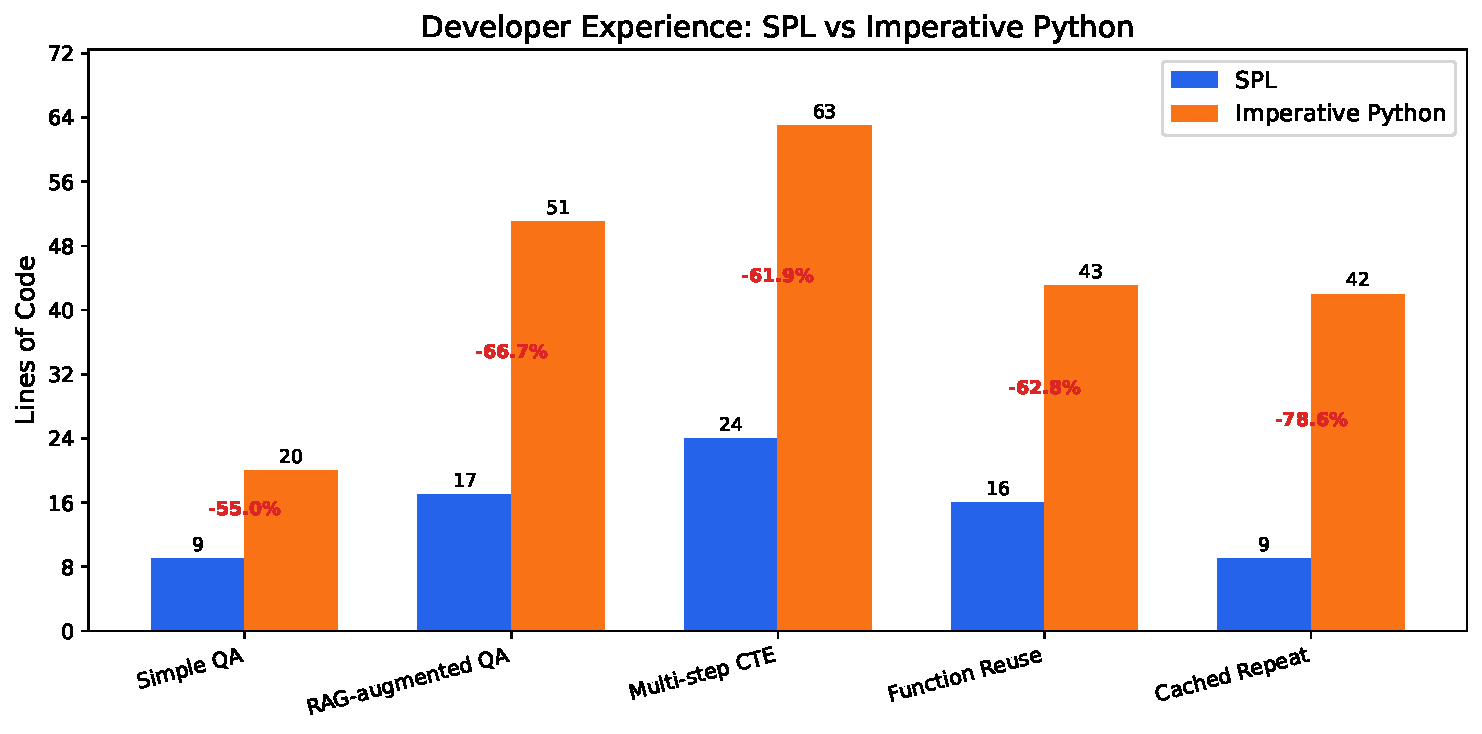
\includegraphics[width=0.85\textwidth]{figures/figure1_loc_comparison.pdf}
\caption{Lines of code comparison: SPL (blue) vs.\ imperative Python (orange). Percentage labels show code reduction. The most dramatic reduction (78.6\%) occurs for cached queries, where SPL provides automatic caching while Python requires manual cache implementation.}
\label{fig:loc-comparison}
\end{figure}

\subsection{Experiment 2: Token Budget Optimization}

We analyze the optimizer's behavior under varying budget levels and increasing context pressure.

\subsubsection{Allocation Under Varying Budgets}

Running the same query structure with budgets from 2K to 32K tokens:

\begin{table}[h]
\centering
\caption{Token allocation strategy adapts proportionally to budget level.}
\label{tab:token-allocation}
\begin{tabular}{@{}rrrrrrrr@{}}
\toprule
\textbf{Budget} & \textbf{System} & \textbf{Question} & \textbf{RAG} & \textbf{Memory} & \textbf{Output} & \textbf{Buffer} & \textbf{Util\%} \\
\midrule
2,000  & 20 & 200 &   666 &   250 &   500 &   364 & 81.8\% \\
4,000  & 20 & 200 & 1,333 &   500 & 1,000 &   947 & 76.3\% \\
8,000  & 20 & 200 & 2,666 & 1,000 & 2,000 & 2,114 & 73.6\% \\
16,000 & 20 & 200 & 5,333 & 2,000 & 4,000 & 4,447 & 72.2\% \\
32,000 & 20 & 200 & 8,000 & 2,000 & 8,000 & 13,780 & 56.9\% \\
\bottomrule
\end{tabular}
\end{table}

The optimizer allocates tokens proportionally: RAG and memory scale with budget while system role and question remain fixed. At 32K, the RAG limit (8K) and memory limit (2K) cap out, leaving substantial buffer---visible to the developer via \texttt{EXPLAIN}.

\begin{figure}[h]
\centering
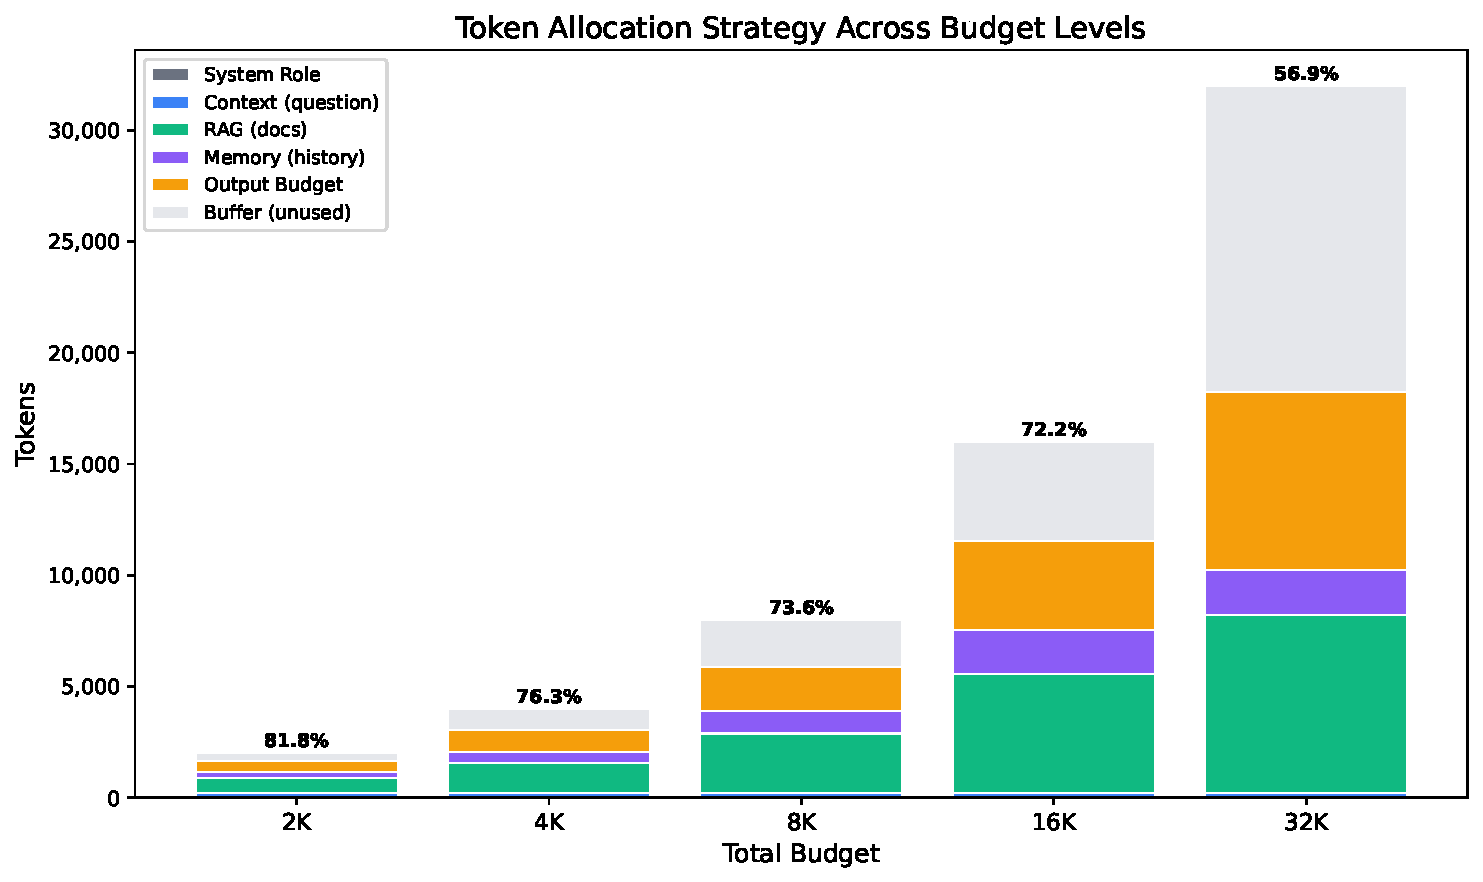
\includegraphics[width=0.85\textwidth]{figures/figure2_token_allocation.pdf}
\caption{Stacked token allocation across budget levels. RAG (green) and memory (purple) scale proportionally; system role and question remain constant. Buffer (gray) grows at high budgets when source limits cap out.}
\label{fig:token-allocation}
\end{figure}

\subsubsection{Compression Under Budget Pressure}

When context demands exceed the budget, the optimizer applies proportional compression (largest items first):

\begin{figure}[h]
\centering
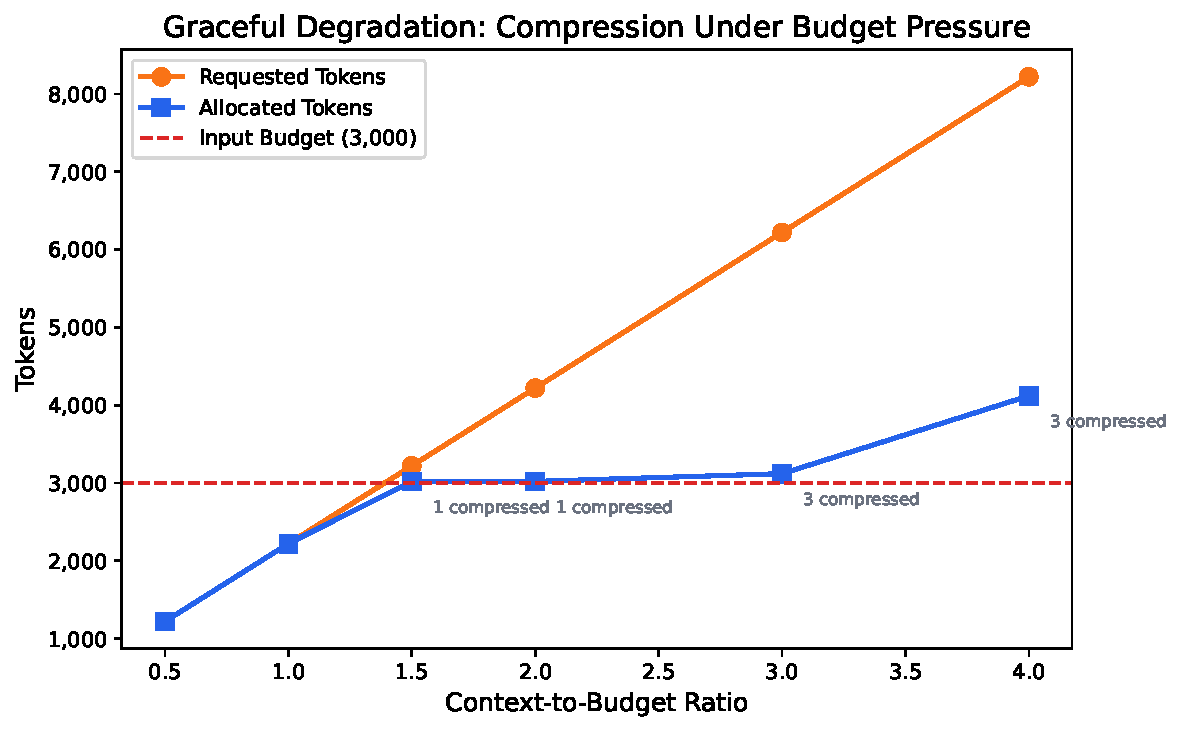
\includegraphics[width=0.75\textwidth]{figures/figure3_compression.pdf}
\caption{Graceful degradation: as context-to-budget ratio increases from 0.5x to 4x, the optimizer increasingly compresses sources to fit within the budget (red dashed line). At 3--4x over-budget, all sources are compressed by 50\%.}
\label{fig:compression}
\end{figure}

At 1.5x over-budget, only the largest source (RAG docs) is compressed. At 3--4x, all sources are compressed proportionally. This behavior is fully transparent via \texttt{EXPLAIN}, which annotates compressed sources with their compression ratio.

\subsection{Experiment 3: Cross-Model Cost Estimation}

SPL's \texttt{EXPLAIN} mechanism provides pre-execution cost estimates. Running the same 8K-budget query across six models:

\begin{table}[h]
\centering
\caption{Pre-execution cost estimation across LLM models (same query, 3,720 input + 2,000 output tokens).}
\label{tab:cost-estimation}
\begin{tabular}{@{}llrrr@{}}
\toprule
\textbf{Model} & \textbf{Tier} & \textbf{Est.\ Cost} & \textbf{Relative} \\
\midrule
GPT-4 (Legacy)     & Legacy Premium &  \$0.2316 & 67.5x \\
Claude Opus 4.6    & Premium        &  \$0.2058 & 60.0x \\
Claude Sonnet 4.5  & Balanced       &  \$0.0412 & 12.0x \\
GPT-4o             & Flagship       &  \$0.0293 &  8.5x \\
GPT-3.5 Turbo      & Budget         &  \$0.0049 &  1.4x \\
Claude Haiku 4.5   & Economy        &  \$0.0034 &  1.0x \\
\bottomrule
\end{tabular}
\end{table}

The \textbf{68x cost difference} between the most and least expensive models is visible \emph{before execution}. No other prompt management framework provides this capability. This is directly analogous to how SQL \texttt{EXPLAIN} reveals that a full table scan costs more than an index lookup---enabling informed optimization.

\begin{figure}[h]
\centering
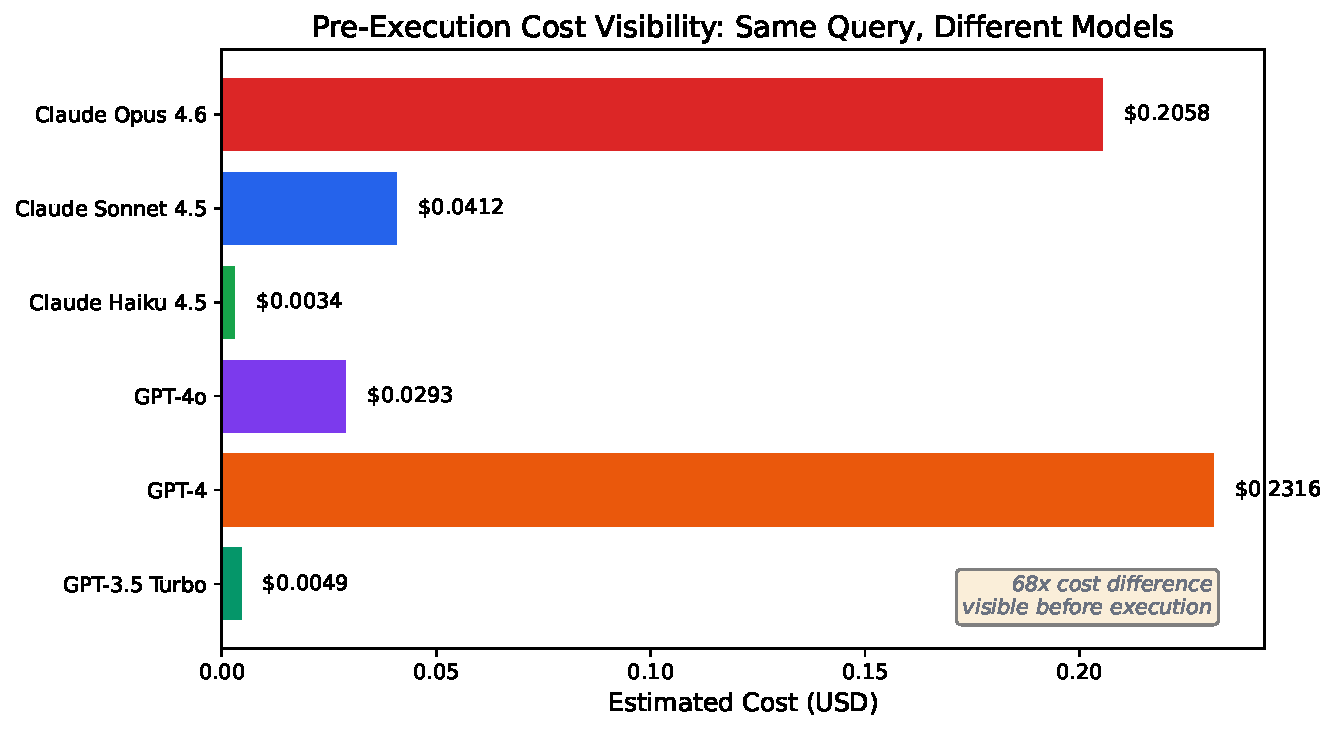
\includegraphics[width=0.8\textwidth]{figures/figure4_cost_comparison.pdf}
\caption{Pre-execution cost comparison across models. The same SPL query costs \$0.0034 on Claude Haiku vs.\ \$0.2316 on GPT-4---a 68x difference visible before any tokens are spent.}
\label{fig:cost-comparison}
\end{figure}

\subsection{Experiment 4: EXPLAIN Output}

The following is the actual \texttt{EXPLAIN} output for the RAG-augmented QA query---the SPL equivalent of SQL's execution plan:

\begin{verbatim}
Execution Plan for: answer_question
============================================================
Budget: 8,000 tokens | Model: claude-sonnet-4-5

Token Allocation:
+-- __system_role__               20 tokens  (  0.2%)
+-- history                      500 tokens  (  6.2%)  [from memory]
+-- docs                       3,000 tokens  ( 37.5%)  [cache MISS]
+-- question                     200 tokens  (  2.5%)
+-- Output Budget              2,000 tokens  ( 25.0%)
\-- Buffer                     2,280 tokens  ( 28.5%)
                               ----------
Total                          5,720 / 8,000 tokens (71.5%)

Estimated Cost: $0.0412
\end{verbatim}

This plan reveals that (1) memory is fetched first (priority ordering), (2) RAG docs consume the largest share (37.5\%), (3) 28.5\% of the budget remains as buffer, and (4) the estimated cost is \$0.04. A developer can inspect this plan, adjust \texttt{LIMIT} values or switch models, and re-run \texttt{EXPLAIN}---all without spending any tokens.

\subsection{Experiment 5: Feature Verification}

We systematically verified all competitive claims from Table~\ref{tab:comparison} by running 20 automated checks against the SPL engine. All 20 checks pass:

\begin{itemize}[nosep]
  \item 4/4 example files parse without error (declarative syntax)
  \item 3/3 token budgeting features work (\texttt{WITH BUDGET}, \texttt{LIMIT}, \texttt{OUTPUT BUDGET})
  \item 3/3 EXPLAIN capabilities verified (tree output, percentages, cost)
  \item 2/2 RAG features work (\texttt{rag.query()} parsing, VectorStore importable)
  \item 2/2 memory features work (\texttt{memory.get()} parsing, MemoryStore importable)
  \item 1/1 CTE support verified (\texttt{WITH ... AS})
  \item 1/1 function support verified (\texttt{CREATE FUNCTION})
  \item 2/2 provider adapters importable (Claude CLI, OpenRouter)
  \item 1/1 automatic compression triggers on over-budget queries
  \item 1/1 zero-dependency parser confirmed (no ANTLR/Lark imports)
\end{itemize}

\subsection{Parser Correctness}

The reference implementation passes a comprehensive test suite of 40 tests:

\begin{itemize}[nosep]
  \item \textbf{Lexer}: 14 tests covering tokenization of keywords, strings, numbers, operators, comments, dot notation, and error cases.
  \item \textbf{Parser}: 20 tests across basic prompts, generate clauses, WHERE clauses, CTEs, STORE clauses, and end-to-end parsing of all example files.
  \item \textbf{Optimizer}: 6 tests covering execution plan generation, token allocation, execution ordering, EXPLAIN output rendering, and over-budget compression.
\end{itemize}

% ============================================================
\section{Limitations and Future Work}
\label{sec:discussion}
% ============================================================

\subsection{Current Limitations}

We acknowledge several limitations of the current SPL prototype:

\begin{enumerate}[nosep]
  \item \textbf{No learned optimization}: SPL's optimizer uses heuristic rules (proportional compression, priority ordering). A learned optimizer---trained on execution traces to predict optimal token allocations---could significantly improve budget utilization.
  \item \textbf{Compression is truncation}: The current compression strategy is simple truncation. More sophisticated compression (summarization via a cheaper model, semantic deduplication) is a direction for future work.
  \item \textbf{Limited type system}: SPL does not yet have a rich type system for context sources. Typed schemas for RAG documents, memory values, and function signatures would improve static analysis.
  \item \textbf{Single-query scope}: SPL currently optimizes individual queries. Multi-query optimization (pipeline-level budget allocation across a sequence of SPL queries) is not yet supported.
\end{enumerate}

\subsection{Learned Optimization}

Current SQL query optimizers use sophisticated cost models and statistics. SPL could benefit from:

\begin{itemize}[nosep]
  \item \textbf{Token allocation learning}: Training a model to predict optimal token allocations based on query structure, source characteristics, and historical performance.
  \item \textbf{Compression strategy selection}: Learning which compression technique (truncation, summarization, extraction) works best for each source type and budget constraint.
  \item \textbf{Model routing}: Automatically selecting the optimal model based on query complexity, required capabilities, and cost constraints.
\end{itemize}

\subsection{RAG Application Case Studies}

The current evaluation measures developer experience, token budget efficiency, and
cost estimation on synthetic benchmark tasks. A natural next step is to evaluate SPL
against real-world RAG applications---for example, document Q\&A, knowledge-base
search, and multi-hop reasoning pipelines.

Proposed case studies include controlled comparisons of the same RAG application
implemented (a) with SPL's declarative \texttt{SELECT}/\texttt{GENERATE} pipeline
and (b) with an equivalent imperative Python implementation, measuring:
retrieval quality (precision@k, recall@k), end-to-end latency, total token consumption,
and lines of code. Such studies would provide stronger empirical grounding for SPL's
claimed benefits and surface failure modes not visible in the current benchmarks.

\subsection{Integration with Existing Ecosystems}

SPL is designed to complement, not replace, existing tools:

\begin{itemize}[nosep]
  \item \textbf{SPL + DSPy}: Use DSPy for content optimization within SPL's token budget framework.
  \item \textbf{SPL + LangChain/LlamaIndex}: Use SPL as a declarative layer on top of existing retrieval and orchestration infrastructure.
  \item \textbf{SPL in IDEs}: Syntax highlighting, autocompletion, and inline \texttt{EXPLAIN} for \texttt{.spl} files in VS Code, JetBrains, etc.
  \item \textbf{SPL for evaluation}: \texttt{EXPLAIN} output as a standard format for prompt auditing and compliance.
\end{itemize}

\subsection{SPL Ecosystem: Four Planned Extensions}

Beyond the core language presented in this paper, we identify four high-value
extensions that build on SPL's foundation:

\begin{enumerate}

  \item \textbf{Natural Language Interface (Text2SPL).}
  Requiring users to write SPL directly raises the adoption barrier for
  non-technical practitioners.  A \emph{Text2SPL} module---which translates a
  free-form English query into a valid SPL script via an LLM---would make SPL
  accessible to domain experts without programming backgrounds.  Preliminary
  experiments show that few-shot prompting with SPL syntax examples produces
  syntactically correct SPL for the majority of common query patterns; a
  validate-and-retry loop further raises the success rate.  The resulting
  pipeline (NL $\to$ SPL $\to$ execute) mirrors the role of natural language
  interfaces in traditional databases~\citep{androutsopoulos1995natural}.

  \item \textbf{Mixture-of-Models Routing (\texttt{USING MODEL auto}).}
  Current SPL requires the author to hard-code a specific model in every
  \texttt{USING MODEL} clause.  A \emph{late-bound routing} extension---written
  \texttt{USING MODEL auto}---would resolve the target model at execution time
  based on the task type inferred from the prompt content.  A routing table maps
  task categories (CJK language, code, European language, mathematics,
  multi-step reasoning, synthesis, general) to the world's best specialist
  model for each category.  This \emph{Mixture-of-Models} (MoM) paradigm
  maximises quality on heterogeneous multi-CTE scripts without requiring the
  developer to know each model's strengths in advance.

  \item \textbf{\texttt{BENCHMARK}: Parallel Model Comparison.}
  Choosing the right model for a given SPL script today requires sequential
  manual testing.  A \texttt{BENCHMARK} construct would run a single SPL script
  against a user-supplied list of models in parallel
  (\texttt{asyncio.gather}), collecting per-model response text, token
  consumption, latency, and cost into a structured JSON report.  This
  transforms model selection from guesswork into an evidence-based,
  reproducible process---analogous to \texttt{EXPLAIN ANALYZE} in PostgreSQL,
  which measures actual versus estimated query costs.

  \item \textbf{Orchestration Layer (SPL-Flow).}
  SPL scripts today are executed in isolation.  An \emph{orchestration layer}
  would compose multiple SPL queries into directed pipelines with branching,
  retries, and delivery targets (synchronous return, async file output, email
  notification).  Such a layer would also integrate the Text2SPL, routing,
  and BENCHMARK extensions into a unified platform accessible through a
  Streamlit UI, a Python API, and a CLI---lowering the barrier to deploying
  SPL-powered applications in production.

\end{enumerate}


% ============================================================
\section{Conclusion}
\label{sec:conclusion}
% ============================================================

We have presented SPL (Structured Prompt Language), a declarative query language for managing LLM context as a constrained resource. By applying the principles that made SQL successful---declarative specification, automatic optimization, composability, portability, and execution plan transparency---SPL transforms prompt engineering from an ad hoc, imperative practice into a structured, optimizable discipline.

SPL's key innovations are:

\begin{enumerate}[nosep]
  \item \textbf{Token budget as first-class concept}: \texttt{WITH BUDGET} and \texttt{LIMIT} clauses make resource constraints explicit and optimizable.
  \item \textbf{Generative knowledge base model}: The \texttt{SELECT}/\texttt{GENERATE} duality captures the fundamental difference between context retrieval and content synthesis.
  \item \textbf{EXPLAIN for LLM queries}: Transparent execution plans enable developers to inspect and optimize token allocation before execution.
  \item \textbf{Integrated context management}: Built-in RAG (FAISS) and memory (SQLite) eliminate the need for external context infrastructure.
\end{enumerate}

Beyond software engineering, SPL lowers the entry barrier for the large community of
data engineers and analysts who already possess deep SQL expertise.
As the author's own transition from data engineering to AI engineering illustrates,
the conceptual leap from \texttt{SELECT} over relational tables to \texttt{PROMPT}/\texttt{SELECT}/\texttt{GENERATE}
over LLM context sources is far smaller than learning a general-purpose programming framework
from scratch.
For the millions of practitioners who think naturally in sets, schemas, and declarative queries,
SPL offers a familiar on-ramp into the GenAI domain---one that preserves and extends their
existing mental models rather than discarding them.

The reference implementation is available as an open-source Python package (\texttt{pip install spl-llm}) at \url{https://github.com/digital-duck/SPL}.

% ============================================================
% References
% ============================================================

\section*{Acknowledgements}

This project was developed through human and AI collaboration: the author provided the vision, domain expertise (20+ years of SQL/Oracle experience), architectural decisions, experimental design and execution, while the AI collaborator provided implementation, code generation, and synthesis.

The author thanks Claude (Anthropic) in particular for its role as an AI development partner throughout
this project. The SPL engine, test suite, and manual drafting were developed
in close collaboration with Claude, whose ability to implement, synthesise, and iterate
on complex system designs substantially accelerated the work. 

The author also thanks the open-source communities behind FAISS, tiktoken, and the
broader Python ecosystem on which SPL depends.

\bibliographystyle{plainnat}
\bibliography{references}

\end{document}
